\documentclass{article}
\usepackage{tikz}
\usepackage{pgfplots}
\pgfplotsset{compat=newest}
\usetikzlibrary{intersections,shapes.geometric, arrows, shadows,external,patterns}
\usetikzlibrary{calc}

\pgfrealjobname{coverpage}


\tikzstyle{arrow} = [thick,->,>=stealth, line width=1pt]
\tikzstyle{darrow} = [thick,<->,>=stealth, line width=1pt]
\begin{document}
	
\beginpgfgraphicnamed{cover}%
\begin{tikzpicture}

\fill[blue!20]  ([shift={(4,-2)}]170:6) arc[radius=6, start angle=170, end angle= 90] --++(4,0) --++(0,1) --++(-4,0) -- ([shift={(4,-2)}]90:7) arc[radius=7, start angle=90, end angle= 170] -- cycle;

\fill[blue!20]  ([shift={(4,-2)}]170:4) arc[radius=4, start angle=170, end angle= 90] --++ (4,0) --++(0,-1) --++(-4,0) -- ([shift={(4,-2)}]90:3) arc[radius=3, start angle=90, end angle= 170] -- cycle;

\fill[gray!20]  ([shift={(4,-2)}]170:4) arc[radius=4, start angle=170, end angle= 90] --++(4,0) --++(0,2) --++(-4,0) -- ([shift={(4,-2)}]90:6) arc[radius=6, start angle=90, end angle= 170] -- cycle;

\fill [red!20](5,2) rectangle(6.5,4);

\draw[thick,dashed] (5,4) -- (5,2);
\draw[thick,dashed] (6.5,4) -- (6.5,2);

%\node (species1) [shape=rectangle,draw,fill=white] at (-1,4.24){
%	\begin{tabular}{c l}
%	\colorbox{gray!30}{}& Road\\
%	\colorbox{blue!20}{}& Sidewalk \\
%	\colorbox{red!20}{}& Crosswalk
%	\end{tabular}
%};


% Reference path	
\draw[orange!40,very thick] ([shift={(4,-2)}]170:5) arc[radius=5, start angle=170, end angle= 90] --++(4,0);

% Top path
\draw[black,thick] ([shift={(4,-2)}]170:6) arc[radius=6, start angle=170, end angle= 90] --++(4,0);

% Bottom path
\draw[black, thick] ([shift={(4,-2)}]170:4) arc[radius=4, start angle=170, end angle= 90] --++(4,0);

\draw[thick,dashed] (5,3.5) -- (6.5,3.5);
\draw[thick,dashed] (5,3) -- (6.5,3);
\draw[thick,dashed] (5,2.5) -- (6.5,2.5);


% Car image
\coordinate (car) at (0,1.7);
\def\thetaCar{45};
\node[opacity=0.6,inner sep=0pt] at (2.3,2.6) {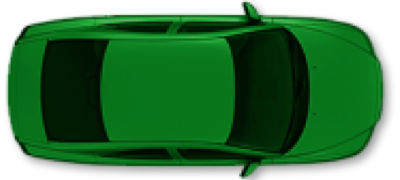
\includegraphics[width=2cm,angle=20]{bil.png}};
\node[opacity=0.6,inner sep=0pt] at (0.6,1.6) {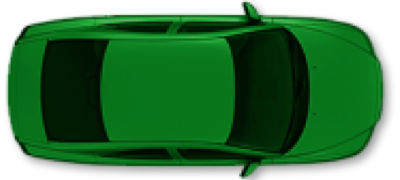
\includegraphics[width=2cm,angle=45]{bil.png}};
\node[opacity=1,inner sep=0pt] at (-0.6,0) {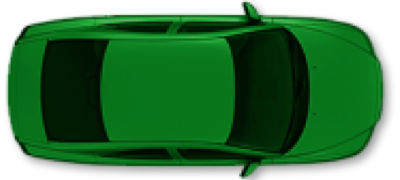
\includegraphics[width=2cm,angle=70]{bil.png}};
%\node[label={$t_3$}] at (1.6,2.8) {};	
%\node[label={$t_2$}] at (0.0,1.5) {};	
%\node[label={$t_1$}] at (-1.2,0) {};	

% Draw region constraints
\draw[opacity=0.5,pattern=north west lines, pattern color = red] (5.75,3.6) circle[radius=1];
\draw[opacity=0.5,pattern=north west lines, pattern color = red] (5.75,2.6) circle[radius=.75];
\draw[pattern=north west lines, pattern color = red] (5.75,1.8) circle[radius=.5];
%\node[label={$t_1$}] at (6.5,1.4) {};	
%\node[label={$t_2$}] at (6.75,2.2) {};	
%\node[label={$t_3$}] at (7,3.3) {};	
% Draw pedestrian
\draw [fill=red!60](5.75,1.8) ellipse (0.4 and 0.2);
\draw [fill=brown!80](5.75,1.8+0.05) ellipse (0.2 and 0.2);

\draw [fill=red!60,opacity=0.6](5.75,2.6) ellipse (0.4 and 0.2);
\draw [fill=brown!80,opacity=0.6](5.75,2.6+0.05) ellipse (0.2 and 0.2);
\draw [fill=red!60,opacity=0.6](5.75,3.6) ellipse (0.4 and 0.2);
\draw [fill=brown!80,opacity=0.6](5.75,3.6+0.05) ellipse (0.2 and 0.2);

%
%\coordinate (xG) at (-1.2,-1);
%\draw[arrow,rotate around={0:(xG)}] (xG) -- +(1,0) node[anchor=north west] {$X_\mathrm{G}$};
%%\draw[arrow,rotate around={0:(xG)}] (xG) -- +(0,1) node[anchor=south east] {$Y_\mathrm{G}$};
%
%\coordinate (xL) at (0,1.7);
%\def\dx{0.5};
%\coordinate (xLRear) at ($(xL)-({\dx*cos(\thetaCar)},{\dx*sin(\thetaCar)})$);
%\draw[arrow,rotate around={\thetaCar:(xLRear)}] (xLRear) -- +(1,0) node[anchor=north west] {$X_\mathrm{L}$};
%\draw[arrow,rotate around={\thetaCar:(xLRear)}] (xLRear) -- +(0,1) node[anchor=south east] {$Y_\mathrm{L}$};

%
%\track{3}{0}{2.5}{1}{1/3}{45}{0};
\end{tikzpicture}
\endpgfgraphicnamed


\end{document}